% ----------------------------------------------------------------
% achemso --- Support for submissions to American Chemical
%  Society journals
% Maintained by Joseph Wright
% E-mail: joseph.wright@morningstar2.co.uk
% Originally developed by Mats Dahlgren
%  (c) 1996-98 by Mats Dahlgren
%  (c) 2007-2008 Joseph Wright
% Released under the LaTeX Project Public license v1.3c or later
% See http://www.latex-project.org/lppl.txt
% 
% Part of this bundle is derived from cite.sty, to which the
% following license applies:
%   Copyright (C) 1989-2003 by Donald Arseneau
%   These macros may be freely transmitted, reproduced, or
%   modified provided that this notice is left intact.
% ----------------------------------------------------------------
% 
% The achemso bundle provides a LaTeX class file and BibTeX style
% file in accordance with the requirements of the American
% Chemical Society.  The files can be used for any documents, but
% have been carefully designed and tested to be suitable for
% submission to ACS journals.
% 
% The bundle also includes the natmove package.  This package is
% loaded by achemso, and provides automatic moving of superscript
% citations after punctuation.

\documentclass[
%journal=ancac3, % for ACS Nano
%journal=acbcct, % for ACS Chem. Biol.
journal=jacsat, % for undefined journal
manuscript=article]{achemso}

\usepackage[version=3]{mhchem} % Formula subscripts using \ce{}
\usepackage[utf8]{inputenc}
\usepackage[T1]{fontenc}
\usepackage[frenchb,english]{babel}

\usepackage{amsmath}

\usepackage{amssymb}

\newcommand*{\mycommand}[1]{\texttt{\emph{#1}}}

\author{Jean Marçais}
%\author{Fred T. Secondauthor}
%\altaffiliation{Current address: Some other place, Othert\"own,
%Germany}
%\author{I. Ken Groupleader}
\email{jean.marcais@gmail.com}
%\affiliation[Unknown University]
%{Géosciences Rennes, Campus de Beaulieu, Université de Rennes 1, 35042 Rennes cedex.}
%\author{Susanne K. Laborator}
%\email{s.k.laborator@bigpharma.co}
%\affiliation[BigPharma]
%{Lead Discovery, BigPharma, Big Town, USA}
%\author{Kay T. Finally}
%\affiliation[Unknown University]
%{Department of Chemistry, Unknown University, Unknown Town}


\title[\texttt{achemso} demonstration]
{Numerical integration of hillslope storage Boussinesq equations}

\begin{document}

%\begin{abstract}
%Lorem ipsum dolor sit amet, consectetur adipiscing elit. Nullam augue odio, placerat quis posuere vel, dictum vitae elit. Proin pharetra ipsum et lacus luctus pellentesque. Aliquam quis tristique nisi. Cum sociis natoque penatibus et magnis dis parturient montes, nascetur ridiculus mus. Nullam eu adipiscing velit. Maecenas tristique varius enim eget lacinia. Duis pretium arcu vitae ipsum tristique suscipit. Praesent sed ante eu nulla sollicitudin vestibulum. Suspendisse auctor risus eget eros adipiscing eget tempus enim imperdiet.
%\end{abstract}


\section{Introduction}

Boussinesq equations are highly non linear and their integration is often done on a variable integration volume. This is due to the fact that free surface of water can going up and intersect the surface. Then the water level is fixed at the surface elevation. 
In this paper we develop a new formulation of the hillslope storage boussinesq equations enabling to take into account the interception of the free surface with the surface. This new formulation is based on the use of Differential Algebraic Equations (DAEs). Indeed use of DAE enable to change from one time step to another the dimension and the type of equation governing the problem. This approach is, as far as we know, new.
%The goal of this paper is to describe how to implement hsB equations in Matlab, following \cite{Troch2003}. In particular the case when the soil is fully saturated is explicitly taken into account.

\subsection{Problem Statement}
Let's consider a sloping aquifer in two dimension (cf. figure \ref{figaquifer}). $h$ denotes the hydraulic head, $h_c$ is the soil/air interface.
Considering the bottom of the aquifer flat, we have the following equations uder the Dupuits-Forchheimer assumption:
\begin{equation}
\label{eqDupuits2D}
\forall t > 0, \forall x \in [0,x_{lim}], \forall y \in [-y_{lim},y_{lim}], \, \,\: \:
\begin{cases}
%\begin{array}{lcl} 
    f \frac{\partial h}{\partial t}  =  \frac{\partial}{\partial x}(k h  \frac{\partial h}{\partial x}) + \frac{\partial}{\partial y}(k h \frac{ \partial h}{\partial y}) + N(t) \\
    h(x,t) \leq h_{c}(x) = d(x)
%\end{array}
\end{cases}
\end{equation}
where k is the hydraulic conductivity and f is the porosity of the aquifer and N is the source term of the equation (efficace rainfall, recharge, infiltration, etc.).

\begin{scheme}
  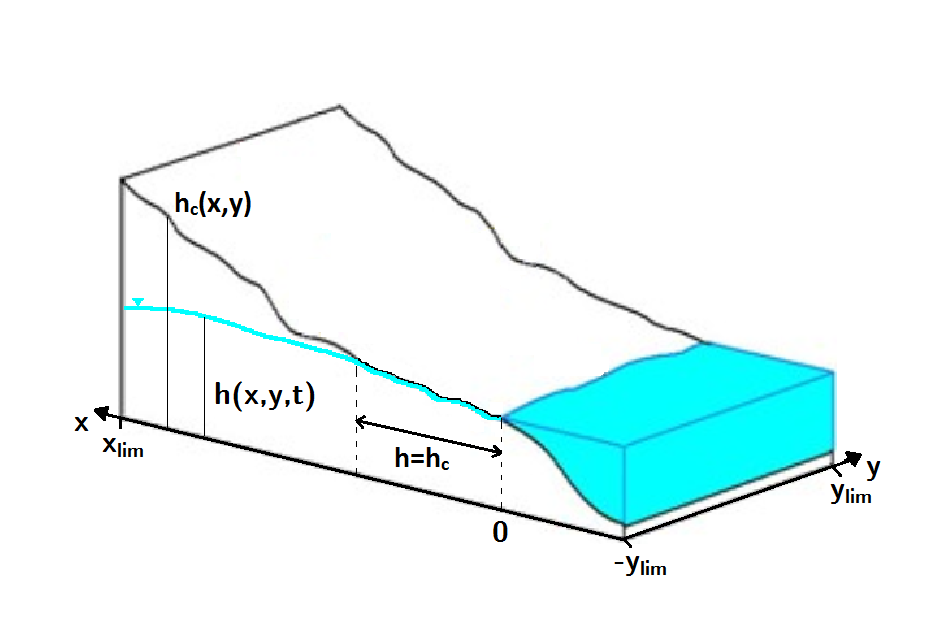
\includegraphics[scale=0.7]{3Dhillslopes3.png}
  \caption{2D hillslope}
  \label{figaquifer}
\end{scheme}

In one dimension, the case where the bottom of the aquifer is not flat can be easily added (cf. figure \ref{figslopingaquifer}). This leads to the following equations:
\begin{equation}
\label{eqDupuits1D}
\forall t > 0, \forall x \in [0,x_{lim}], \, \,\: \:
\begin{cases}
%\begin{array}{lcl} 
    \frac{\partial h}{\partial t}  =  -\frac{\partial Q}{\partial x} + N(t) \\
    Q  =  - kh(\cos i \frac{\partial h}{\partial x}+\sin i) \\
    h(x,t) \leq h_{c}(x) = d(x)
%\end{array}
\end{cases}
\end{equation}
where $Q$ is the Darcy flux and $d$ is the maximum potential thickness of the aquifer. If we are interested in subsurface flow, d is typically the soil depth, subsurface flow taking place in the first meter under ground. Here the reference for h is different from equation \ref{eqDupuits2D}. The reference for h is set at the bottom of the aquifer, having an elevation varying with depth.

\begin{scheme}
  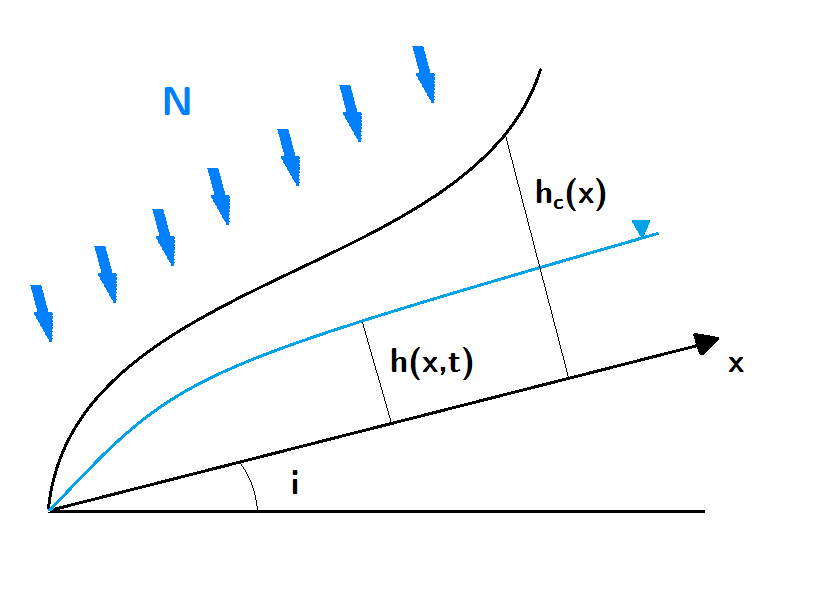
\includegraphics[scale=0.7]{hillslopes.png}
  \caption{1D hillslope. Adapted from \citet{Troch2003}.}
  \label{figslopingaquifer}
\end{scheme}

Following \citet{Troch2003}, we can rewrite this problem by considering the soil moisture storage $S=fwh$ instead of the hydrauilc head $h$. $w$ represents the width function \citet{FanBras}. The width function $w$ characterize for a given position x the width of one hillslope (cf. figure \ref{widthfunctionTroch}).

\begin{scheme}
  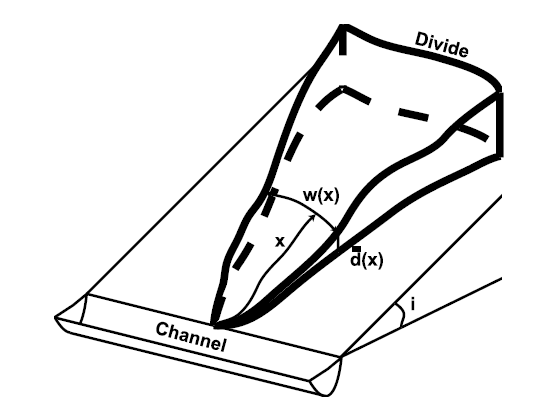
\includegraphics[scale=0.7]{widthfunction.png}
  \caption{Width function visualization. Taken from \citet{Troch2003}.}
  \label{widthfunction}
\end{scheme}

This enables us to aggregate the response of a 2 dimensional aquifer into one dimension by writing the following equation on $S$ and $Q$.  
This leads to the so called hillslope storage Boussinesq equations:
\begin{equation}
\label{eqhsB}
\forall t > 0, \forall x \in [0,x_{lim}] \, \,\: \:
\begin{cases}
%\begin{array}{lcl} 
    \frac{\partial S}{\partial t}  =  -\frac{\partial Q}{\partial x} + N(t)w(x) \\
    Q  =  -\frac{kS}{f}(\cos i \frac{\partial}{\partial x}\frac{S}{fw}+\sin i) \\
    S(x,t) \leq S_{c}(x) = f w(x) d(x)
%\end{array}
\end{cases}
\end{equation}
Note that the angle $i$ can vary with the distance to the stream ($x=0$), i.e. $i=i(x)$. 

We can add Dirichlet boundary condition at $x=0$ and Neumann's at $x=x_{lim}$: 
\begin{equation}
\begin{cases}
    S(x=0,t)=0 \\
    Q(x=x_{lim},t)=0
\end{cases}
\end{equation}

Finally, we can consider two types of initial conditions:
\begin{equation}
\begin{cases}
    S(x,t=0)=0 \\ 
    Q(x,t=0)=0
\end{cases}
\end{equation}

or 
\begin{equation}
\begin{cases}
    S(x,t=0)=R \cdot S_{c}(x) \\ 
    Q(x,t=0)=-\frac{k}{f}S_{t=0}\cdot (\cos i \frac{\partial}{\partial x}(\frac{S}{fw})\big|_{t=0}+\sin i)
\end{cases}
\end{equation}
where $R$ represents the percentage of how much the hillslope is loaded.

\subsection{Transforming the problem into a DAE}
What is typically done with equation \ref{eqhsB}, is to replace $Q$ by its Darcy expression. So the system reduces to the equation on $S$:
\begin{equation}
\begin{cases}
        f\frac{\partial S}{\partial t}  =  \frac{k \cos i}{f}(\frac{\partial}{\partial x}\big(\frac{S}{w}(\frac{\partial S}{\partial x}-\frac{S}{w}\frac{\partial w}{\partial x})\big) + k\sin i \frac{\partial S}{\partial x} +fNw \\
        S(x,t) \leq S_{c}(x) = f w(x) d(x)
\end{cases}
\end{equation}

What we develop here is a code that computes both $S$ and $Q$ and stays with a formulation that separates conservation equation and Darcy flux equation. The major advantage of this formulation is to exactly conserve the mass in a finite difference scheme. The code also gains in clarity and computation's time with this formulation as it is obvious to write equations in a vectorized form. 

The second thing is to transform the condition that prevent soil moisture storage to go over the maximal value $S_c$. To do this and in order to conserve mass in the equation we can consider the flux $q_{S}(x,t)$ which represents the flux going out of the soil if $S(x,t) = S_{c}(x)$. 

Basically the idea is to partition the flux balance (flux entering minus flux exiting) of a given spatial domain between one part that goes to the variation of $\frac{\partial S}{\partial t}$ and another that go to the outflow flux $q_S$. Obviously, the partition's ratio depends on the value of $S$ compared to $S_c$ and on values of $\frac{\partial S}{\partial t}$.

We define: 
\begin{equation}
    q_{in}-q_{out}=-\frac{\partial Q}{\partial x} + N w
\end{equation}
Mathematically we have
\begin{equation}
\begin{cases}
    \frac{\partial S}{\partial t}  = \alpha \cdot (q_{in}-q_{out}) \\
    q_{S}= (1-\alpha) \cdot (q_{in}-q_{out})
\end{cases}
\end{equation}
where $\alpha$ is defined as
\begin{equation}
    \alpha=\begin{cases}
    1 \; \; \;  \; \; \; \textnormal{if}  \; \; \;  \; \; \; \; \; \; \: \frac{\partial S}{\partial t}<0 \; \; \; \; \; \; || \; \; \; \; \; \; S<S_c\\
    0 \; \; \;  \; \; \; \textnormal{if} \; \; \;  \; \; \; \; \; \; \: \frac{\partial S}{\partial t}\geqslant 0 \; \; \; \; \; \;   \& \; \; \; \; \; \; S=S_c
    \end{cases} 
\end{equation}

To do this we introduce the sigmoid g (see figure \ref{sigmoid}):
\begin{equation}
   \forall z \in [0,1] \: \: \: g(z)=1-\frac{1}{1+\exp (-300*(z-0.95))}
\end{equation}
and the function test h
\begin{equation}
   \forall z \in [0,1] \: \: \: h(z)=\begin{cases}
   1  \; \; \; \textnormal{if} \; \; \; z\geqslant0 \\
   0  \; \; \; \textnormal{if} \; \; \; z <0
   \end{cases}
\end{equation}
$\alpha$ becomes 
\begin{equation}
   \alpha=g\big(\frac{S}{S_{c}}\big)\cdot h\big(\frac{\partial S}{\partial t}\big) + \bigg(1-h\big(\frac{\partial S}{\partial t}\big)\bigg)
\end{equation}

\begin{scheme}
  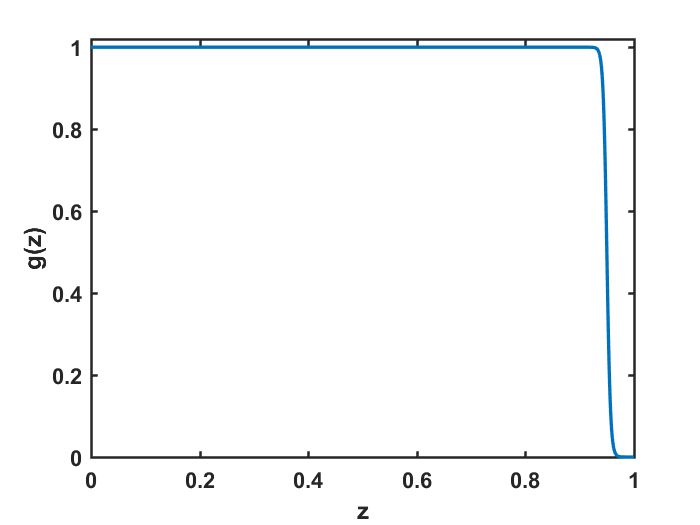
\includegraphics[scale=0.6]{sigmoid.png}
  \caption{Sigmoid}
  \label{sigmoid}
\end{scheme}


Finally, equation \ref{eqhsB} becomes: 
\begin{equation}
\begin{cases}
    \frac{\partial S}{\partial t}  = \alpha \cdot (-\frac{\partial Q}{\partial x} + N w) \\
    Q  =  -\frac{kS}{f}(\cos i \frac{\partial}{\partial x}\frac{S}{fw}+\sin i) \\
    q_{S}= (1-\alpha) \cdot (-\frac{\partial Q}{\partial x} + N w)
\end{cases}
\end{equation}

After some arrangements, the system can be written like this:
\begin{equation}
\label{hsBfluxout}
    \begin{cases}
\begin{array}{ccccccccc} 
    \frac{\partial S}{\partial t}  & = &  & - & \alpha \cdot \frac{\partial Q}{\partial x} &  &  & + & \alpha \cdot Nw \\
    0 & = &P(S) \cdot S & + & Q & & & &\\
    0 & = & & - & (1-\alpha) \cdot \frac{\partial Q}{\partial x} & - &  q_{s} & + & (1-\alpha) \cdot Nw
\end{array}
\end{cases}
\end{equation}

where $ P(S)=\frac{k}{f}(\cos i \frac{\partial}{\partial x}\frac{S}{fw}+\sin i)$.


Finally to prevent $S$ to become negative, one can add a $\beta$ coefficient to equation \ref{hsBfluxout} so that if $\frac{\partial S}{\partial t}<0$ \& $S=0$ then $\frac{\partial S}{\partial t}=0$ for the next time step. We have 
\begin{equation}
    \beta=1-\delta\big(S\big) \cdot \bigg(1-h\big(\frac{\partial S}{\partial t}\big)\bigg)
\end{equation}
where $\delta$ is the dirac function.

The DAE we consider is finally:
\begin{equation}
\label{hsBfluxout2}
    \begin{cases}
\begin{array}{ccccccccc} 
    \frac{\partial S}{\partial t}  & = &  & - & \alpha \cdot \beta \cdot \frac{\partial Q}{\partial x} &  &  & + & \alpha \cdot \beta \cdot Nw \\
    0 & = &P(S) \cdot S & + & Q & & & &\\
    0 & = & & - & (1-\alpha) \cdot \frac{\partial Q}{\partial x} & - &  q_{s} & + & (1-\alpha) \cdot Nw
\end{array}
\end{cases}
\end{equation}

\subsection{Space Discretization}
Let's now discretize the system \ref{hsBfluxout2} in space. Consider $N_{x} \in \mathbb{N}^{+}$.
We define $ \Delta x= x_{lim} / N_{x}$ and $\forall i \in \mathbb{N} \: \: S_{i}(t)=S(x_{i},t)=S(i\cdot \Delta x,t)$. Similar notations are used for $Q$ and $q_{s}$.

Now we have:
\begin{equation}
S=
\begin{bmatrix}
    S_{0} \\
    S_{1} \\
    \vdots \\
    S_{N_{x}} \\
\end{bmatrix} \, , \: \: \:
Q=
\begin{bmatrix}
    Q_{0} \\
    Q_{1} \\
    \vdots \\
    Q_{N_{x}} \\
\end{bmatrix} \: \: \:  \& \: \: \:
q_{s}=
\begin{bmatrix}
    {q_{s}}_{0} \\
    {q_{s}}_{1} \\
    \vdots \\
    {q_{s}}_{N_{x}} \\
\end{bmatrix}
\end{equation}

Discretization in space leads to:
\begin{equation}
    \frac{\partial Q}{\partial x}=\frac{A}{2 \Delta x}\cdot Q, \: \: where \: \:  A=
    \begin{pmatrix}
    0 & 1 & 0 & \ldots & 0 \\
    -1 & \ddots & \ddots & \ddots & \vdots \\
    0 & \ddots & \ddots & \ddots & 0 \\
    \vdots & \ddots & \ddots & \ddots & 1 \\
    0 & \ldots & 0 & -1 & 0 \\
    \end{pmatrix}
\end{equation}

and 
\begin{equation}
    \frac{\partial S}{\partial x}=\frac{B}{\Delta x}\cdot S, \: \: where \: \:  B=
    \begin{pmatrix}
    -1 & 1 & 0 & \ldots & 0 \\
    0 & \ddots & \ddots & \ddots & \vdots \\
    \vdots & \ddots & \ddots & \ddots & 0 \\
    \vdots &  & \ddots & \ddots & 1 \\
    0 & \ldots & \ldots & 0 & -1 \\
    \end{pmatrix}
\end{equation}

and 
\begin{equation}
    \frac{S(x)+S(x+\Delta x)}{2}=\Omega \cdot S, \: \: where \: \:  \Omega=
    \begin{pmatrix}
    0.5 & 0.5 & 0 & \ldots & 0 \\
    0 & \ddots & \ddots & \ddots & \vdots \\
    \vdots & \ddots & \ddots & \ddots & 0 \\
    \vdots &  & \ddots & \ddots & 0.5 \\
    0 & \ldots & \ldots & 0 & 0.5 \\
    \end{pmatrix}
\end{equation}


Let y now denote the column vector: $\begin{bmatrix}
    S \\
    Q \\
    q_{s} \\
\end{bmatrix}$. We have now a differential algebraic equation (DAE):
\begin{equation}
    M \cdot \frac{\partial y}{\partial t}=C \cdot y + D
\end{equation} where M is the mass matrix defined by:
\begin{equation}
M=
\left[
\begin{array}{c|c|c}
I_{N_{x}+1} & \; \; \; 0 \; \; \;  &\; \;  \; 0\;   \; \;  \\
\hline
0 & 0 & 0 \\
\hline
0 & 0 & 0
\end{array}
\right]
\end{equation}

C is defined by:
\begin{equation}
C=
\left[
\begin{array}{c|c|c}
0 & -\frac{A}{2 \Delta x}  & -I_{N_{x}+1}  \\
\hline
P(S) & \Omega & 0 \\
\hline
0 & R(S) & I_{N_{x}+1}
\end{array}
\right]
\end{equation}
where:
\begin{equation}
\begin{array}{rcl}
     R(S) & = &  \frac{1}{2 \Delta x} \cdot diag(1-g(\frac{S}{fdw}))\cdot A\\
     %and \: \: \: \: \: \: \: \: P(S) & = & \frac{k}{f}(\cos i \frac{B}{\Delta x}\frac{S}{fw}+\sin i+\frac{\cos i}{f \Delta x}\frac{S_{N_{x}+1}}{w_{N_{x}+1}})
     and \: \: \: \: \: \: \: \: P(S) & = & \frac{k}{f}(\cos i \frac{B}{\Delta x}\frac{S}{fw}+\sin i) \cdot \Omega
\end{array}
\end{equation}

and D by:
\begin{equation}
    D=
    \begin{bmatrix}
        %Nw+\frac{Q_{-1}}{2 \Delta x} \\
        Nw\\
        0 \\
        %-diag(1-g(\frac{S}{fdw}))\cdot (Nw+\frac{Q_{-1}}{2 \Delta x}) \\
        -diag(1-g(\frac{S}{fdw}))\cdot Nw \\
    \end{bmatrix}
\end{equation}


\bibliography{sample}

\end{document}
